% Provenance (never printed): enseignement scientifique premiere (2019),
% theme "La Terre, un astre singulier: la forme de la Terre" (Eratosthenes,
% meridian measurement by triangulation, the metre); see
% sources/book2/PROVENANCE.md. Every length on the ellipsoid is computed in
% figdata/grade-10/meridian_degree.py (WGS 84, ledger wgs84:ellipsoid).
\chapter{Mengukur Bumi}\label{ch:g10:measuring-the-earth}

Berdirilah di pantai dan perhatikan sebuah kapal yang berlayar menjauh ke
laut lepas. Kapal itu tidak sekadar mengecil sampai terlalu kecil untuk
dilihat: mula-mula lambungnya menghilang, seakan-akan tenggelam, lalu bagian
bawah bangunan atasnya, dan puncak tiangnya hilang paling akhir. Laut di
antara kamu dan kapal itu tidak datar; permukaannya menggembung. Lebih dari
dua puluh dua abad yang lalu, seorang cendekiawan dari Aleksandria mengubah
pengamatan yang serupa --- panjang bayang-bayang pada tengah hari --- menjadi
pengukuran ukuran seluruh planet. Bab ini mengikuti pengukuran itu dan
pengukuran-pengukuran sesudahnya: rantai segitiga yang dibentangkan para juru
ukur melintasi negeri-negeri, ekspedisi yang dikirim ke Arktik dan ke
khatulistiwa untuk mengetahui apakah Bumi pepat, lahirnya meter, dan satelit
yang kini dipakai untuk mengukur planet ini.

\begin{omfigure}
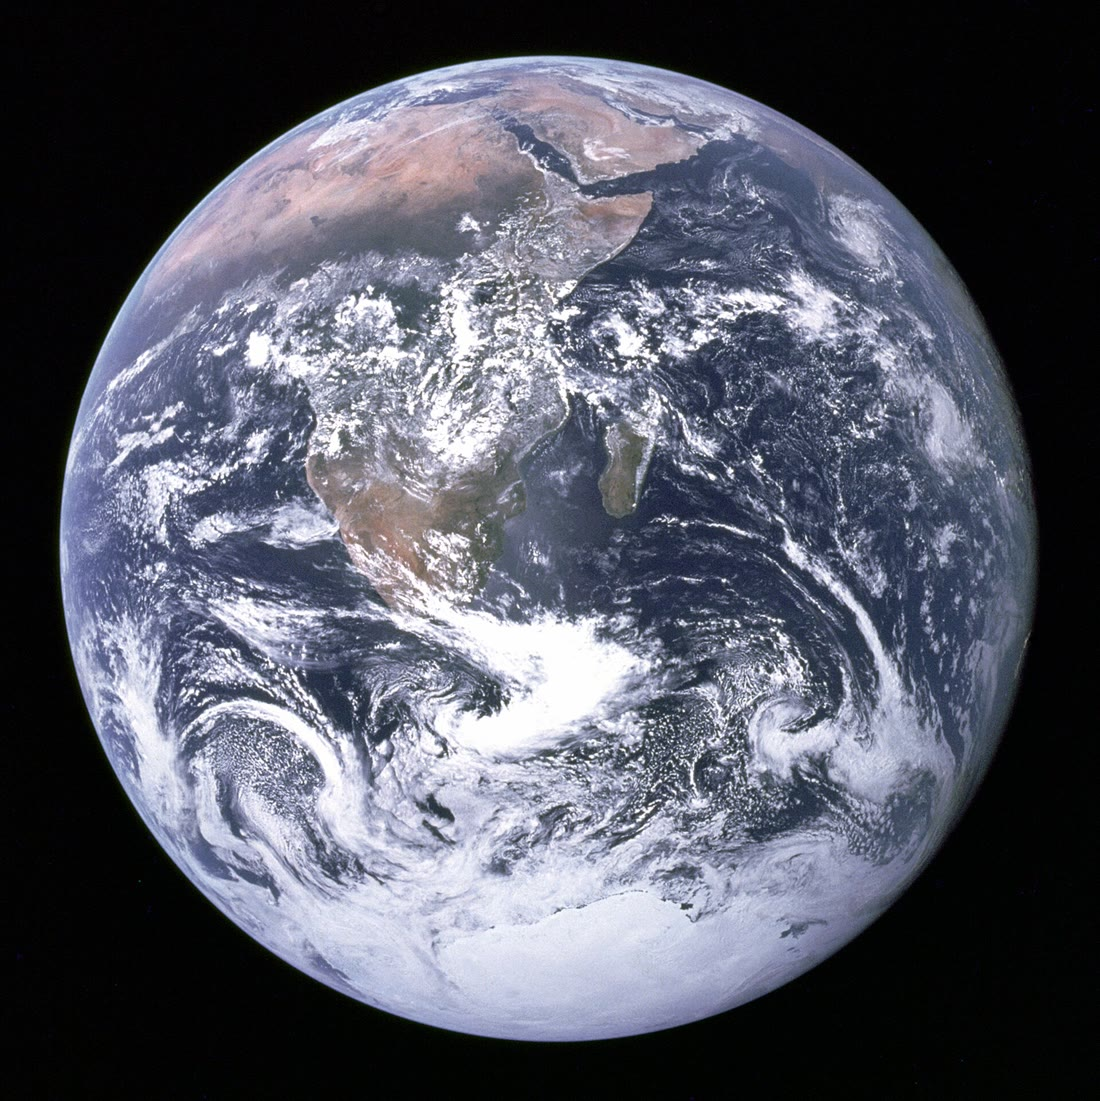
\includegraphics[width=0.5\linewidth]{images/book2/g10-nasa-apollo17-earth.jpg}

{\small Bumi yang dipotret oleh awak Apollo~17 dalam perjalanan menuju Bulan,
pada Desember 1972: Afrika, Jazirah Arab, dan es Antarktika. Foto:
NASA (domain publik).}
\end{omfigure}

\begin{recall}
Letak suatu tempat di Bumi ditentukan oleh lintangnya, yaitu sudutnya ke utara
atau ke selatan dari khatulistiwa, dan bujurnya, yaitu sudutnya ke timur atau
ke barat dari sebuah meridian acuan; meridian menghubungkan kedua kutub,
sedangkan paralel melingkari Bumi sejajar dengan khatulistiwa (Buku 1). Dalam
medium yang seragam cahaya merambat lurus, dan sinar yang sampai di Bumi dari
Matahari yang sangat jauh saling sejajar (buku-buku fisika). Dalam segitiga
siku-siku, sinus sebuah sudut lancip adalah sisi depan dibagi sisi miring,
kosinusnya sisi samping dibagi sisi miring, dan tangennya sisi depan dibagi
sisi samping (buku-buku matematika).
\end{recall}

\section{Bumi yang bulat}

Jauh sebelum ada orang yang dapat melihat Bumi dari angkasa, beberapa
pengamatan sudah menunjukkan bahwa Bumi itu bulat.
\begin{itemize}
  \item \textbf{Kapal di balik cakrawala.} Kapal yang berlayar menjauh
        menghilang dari bawah ke atas, ke segala arah dan di setiap laut:
        permukaan laut melengkung di mana-mana.
  \item \textbf{Bayang-bayang di Bulan.} Saat gerhana Bulan, bayang-bayang
        Bumi jatuh pada Bulan. Tepinya selalu berupa busur lingkaran, pada jam
        berapa pun malam itu; hanya bola yang menghasilkan bayang-bayang bulat
        ke segala arah.
  \item \textbf{Bintang-bintang berubah menurut lintang.} Seorang pelancong
        yang bergerak ke utara melihat Bintang Utara naik makin tinggi di atas
        cakrawala, sedangkan bintang-bintang langit selatan tenggelam di
        bawahnya: cakrawala pelancong itu miring karena ia bergerak di atas
        permukaan yang melengkung.
  \item \textbf{Pelayaran keliling dunia dan pemandangan dari angkasa.}
        Kapal-kapal, lalu pesawat terbang, telah mengelilingi dunia ke segala
        arah; sejak tahun 1960-an seluruh planet yang bulat ini telah dipotret.
\end{itemize}

\begin{omfigure}
\begin{tikzpicture}[font=\small, >={Stealth[length=2.2mm]}]
  % sea surface: arc of a circle of radius 8 centred at (0,-8) (curvature exaggerated)
  \fill[omDef!10] plot[domain=-4.6:4.6, samples=60] (\x,{sqrt(64-\x*\x)-8}) -- (4.6,-2.2) -- (-4.6,-2.2) -- cycle;
  \draw[omDef!70!black, thick] plot[domain=-4.6:4.6, samples=60] (\x,{sqrt(64-\x*\x)-8});
  % observer on a small tower at x=-4 (surface y=-1.072), eye at y=-0.235
  \draw[black!70, line width=1pt] (-4,-1.072) -- (-4,-0.235);
  \fill (-4,-0.235) circle (2pt);
  \node[anchor=east, align=right] at (-4.1,-0.2) {mata\\pengamat};
  % line of sight tangent at x=-0.5 (y=-0.0156, slope 0.0626)
  \draw[omThm!80!black, thick] (-4,-0.235) -- (4.4,0.290);
  \node[omThm!80!black, anchor=south, rotate=3.6] at (1.3,0.1) {garis pandang};
  \fill[omThm!80!black] (-0.5,-0.0156) circle (1.4pt);
  % ship at x=3 (surface y=-0.584), tilted 22 degrees with the local vertical
  \begin{scope}[shift={(3,-0.584)}, rotate=-22]
    \fill[black!12] (-0.6,0) -- (0.6,0) -- (0.75,0.32) -- (-0.75,0.32) -- cycle;
    \draw[black!45, densely dashed] (-0.6,0) -- (0.6,0) -- (0.75,0.32) -- (-0.75,0.32) -- cycle;
    \draw[black!45, densely dashed] (0,0.32) -- (0,0.95);
    \draw[black!80, line width=1pt] (0,0.95) -- (0,1.55);
    \fill[black!80] (0,1.55) -- (0.32,1.25) -- (0,1.25) -- cycle;
  \end{scope}
  \node[anchor=north, align=center, font=\footnotesize] at (2.9,-1.25) {lambung dan tiang bawah\\tertutup tonjolan laut};
  \node[anchor=north, font=\footnotesize] at (-0.5,-0.1) {cakrawala};
\end{tikzpicture}

{\small Mengapa kapal menghilang dari bawah ke atas: pengamat hanya melihat
apa yang berada di atas garis pandang yang menyinggung laut di cakrawala.
Kelengkungannya sangat dibesar-besarkan.}
\end{omfigure}

\section{Eratosthenes mengukur Bumi}

Eratosthenes dari Kirene (276--194 SM) adalah pustakawan Aleksandria. Ia
mendengar bahwa di Syene, kini Aswan, jauh di hulu Sungai Nil, Matahari
menerangi seluruh dasar sebuah sumur pada tengah hari di hari titik balik
musim panas: saat itu Matahari tepat berada di atas kepala. Di Aleksandria,
pada saat yang sama, sebatang tongkat tegak membentuk bayang-bayang pendek:
sinar Matahari membentuk sudut sekitar \qty{7.2}{\degree} dengan garis
vertikal, seperlima puluh lingkaran penuh.
% ledger: erat:method, erat:stadion

\begin{omfigure}
\begin{tikzpicture}[font=\small, >={Stealth[length=2.2mm]}]
  \def\R{2.4}
  \fill[omDef!8] (0,0) circle (\R);
  \draw[omDef!70!black, thick] (0,0) circle (\R);
  \coordinate (O) at (0,0);
  \coordinate (S) at (\R,0);
  \coordinate (A) at ({\R*cos(25)},{\R*sin(25)});
  \coordinate (T) at ({(\R+0.75)*cos(25)},{(\R+0.75)*sin(25)});
  \coordinate (T2) at ({(\R+1.75)*cos(25)},{(\R+1.75)*sin(25)});
  % radii
  \draw[black!70] (O) -- (S);
  \draw[black!70] (O) -- (A);
  \draw[black!40, densely dashed] (A) -- (T2);
  \fill (O) circle (1.5pt) node[below left] {pusat};
  % stick at Alexandria, along the radius
  \draw[line width=1.6pt, black!85] (A) -- ($(A)!0.6!(T)$);
  % well at Syene
  \draw[black!80, thick] ({\R-0.38},-0.12) -- (\R,-0.12) ($(S)+(0,0.12)$) -- ({\R-0.38},0.12);
  % parallel sun rays coming from the right
  \foreach \y in {-1.6,-0.8,0.8,1.6} \draw[->, omThm!70, thick] (6.6,\y) -- (4.4,\y);
  \draw[->, omThm!85!black, thick] (6.6,0) -- (\R+0.05,0);
  \draw[->, omThm!85!black, thick] (6.6,{(\R+0.45)*sin(25)}) -- ({(\R+0.45)*cos(25)+0.03},{(\R+0.45)*sin(25)});
  \node[omThm!85!black, align=center, anchor=west] at (4.6,2.35) {sinar Matahari:\\berkas sejajar};
  % angles
  \draw[omExo!80!black, thick] (0.75,0) arc (0:25:0.75);
  \node[omExo!80!black] at (1.05,0.22) {$\alpha$};
  \coordinate (Q) at ($(A)!0.6!(T)$);
  \draw[omExo!80!black, thick] ($(Q)+(0.8,0)$) arc (0:25:0.8);
  \node[omExo!80!black] at ($(Q)+({1.08*cos(12.5)},{1.08*sin(12.5)})$) {$\alpha$};
  \node[anchor=east] at ($(A)+(-0.12,0.18)$) {Aleksandria};
  \node[anchor=north west] at ($(S)+(0.3,-0.12)$) {Syene};
  \node[font=\footnotesize, anchor=north] at ($(O)!0.5!(S)+(0.2,-0.05)$) {};
  \draw[<->, black!60] ({(\R-0.3)*cos(3)},{(\R-0.3)*sin(3)}) arc (3:22:{\R-0.3});
  \node[anchor=east, font=\footnotesize] at ({(\R-0.35)*cos(13)},{(\R-0.35)*sin(13)}) {$d$};
\end{tikzpicture}

{\small Penalaran Eratosthenes. Di Syene Matahari tepat di atas kepala:
sinarnya mengarah ke pusat Bumi. Di Aleksandria sebatang tongkat tegak, yang
juga mengarah ke pusat, membentuk sudut $\alpha$ dengan sinar Matahari. Sudut
di pusat antara kedua tempat itu sama dengan $\alpha$. Sudutnya
dibesar-besarkan: sebenarnya hanya \qty{7.2}{\degree}.}
\end{omfigure}

\begin{proposition}[Hubungan Eratosthenes]\label{prop:g10:measuring-the-earth:eratosthenes}
Jika dua tempat terletak pada meridian yang sama, berjarak $d$, dan sudut
sinar Matahari tengah hari terhadap garis vertikal di kedua tempat berbeda
sebesar $\alpha$ (dalam derajat), keliling Bumi adalah
\[
  C = \frac{\qty{360}{\degree}}{\alpha}\, d .
\]
\end{proposition}

\begin{proof}
Matahari begitu jauh sehingga sinarnya yang sampai di kedua tempat saling
sejajar. Di setiap tempat, garis vertikal mengarah ke pusat Bumi. Pada gambar,
sinar yang mengenai tongkat dan jari-jari yang melalui Syene adalah dua garis
sejajar, dan jari-jari yang melalui Aleksandria memotong keduanya: sudut
$\alpha$ antara tongkat dan sinar serta sudut di pusat antara kedua jari-jari
adalah sudut-sudut berseberangan, jadi sama besar. Busur $d$ merupakan bagian
dari seluruh keliling yang sama dengan bagian sudut $\alpha$ dari satu putaran
penuh: $d/C = \alpha/\qty{360}{\degree}$.
\end{proof}

\begin{method}[Mengukur keliling dari dua bayang-bayang]\label{met:g10:measuring-the-earth:shadows}
\begin{enumerate}
  \item Pilih dua tempat yang (hampir) terletak pada meridian yang sama, lalu
        ukur jarak utara--selatan $d$ di antara keduanya.
  \item Pada tengah hari setempat di hari yang sama, ukur di setiap tempat
        sudut antara sebatang tongkat tegak dan sinar Matahari:
        $\tan \theta = s/h$, dengan $h$ tinggi tongkat dan $s$ panjang
        bayang-bayangnya. Jangan pernah memandang Matahari itu sendiri: sudut
        dibaca dari bayang-bayang saja.
  \item Ambil selisih $\alpha$ kedua sudut itu dan terapkan
        $C = (360/\alpha)\,d$.
\end{enumerate}
\end{method}

\begin{example}[Angka-angka Eratosthenes]\label{ex:g10:measuring-the-earth:numbers}
% ledger: erat:method, erat:stadion
Eratosthenes menganggap jarak dari Aleksandria ke Syene 5000
\emph{stadion}, sebuah satuan panjang Yunani. Dengan $\alpha = 1/50$ lingkaran,
\[
  C = 50 \times 5000 = 250\,000 \text{ stadion}.
\]
Berapa panjang satu stadion? Para sejarawan masih memperdebatkannya. Dengan
\qty{157.2}{m}, $C \approx \qty{39300}{km}$; dengan \qty{166.7}{m},
$C \approx \qty{41700}{km}$. Keliling meridian yang sebenarnya adalah
\qty{40008}{km}: bagaimanapun juga, hasil Eratosthenes hanya meleset beberapa
persen.
\end{example}

\begin{remark}[Apa yang dianggap benar]\label{rem:g10:measuring-the-earth:assumptions}
Eratosthenes menganggap Bumi berbentuk bola, Matahari cukup jauh sehingga
sinarnya sejajar, Syene tepat berada di garis balik (tempat Matahari dapat
berada tepat di atas kepala), dan Syene tepat di sebelah selatan Aleksandria.
Masing-masing anggapan itu hampir benar, tetapi tidak tepat: Aswan terletak
sekitar \qty{3}{\degree} bujur di sebelah timur Aleksandria. Yang penting
adalah komponen utara--selatan jarak itu, yaitu komponen sepanjang meridian.
% ledger: geonames:aswan, geonames:alexandria
\end{remark}

\section{Triangulasi}

Mengukur jarak yang panjang di tanah dengan rantai atau tongkat ukur berjalan
lambat, dan melintasi sungai, hutan, dan pegunungan hal itu mustahil.
Sebaliknya, sudut dapat diukur dengan sangat teliti memakai teleskop pada
lingkaran berskala, yang diarahkan bergantian ke dua tanda yang jauh. Sejak
abad kedelapan belas, para juru ukur memakai cara ini untuk mengukur seluruh
negeri.

\begin{definition}[Geodesi]\label{def:g10:measuring-the-earth:geodesy}
Yang disebut \emph{geodesi}\index{geodesi} adalah ilmu yang mengukur bentuk
dan ukuran Bumi serta posisi titik-titik di permukaannya, dan mengikuti
perubahannya dari waktu ke waktu.
\end{definition}

\begin{definition}[Triangulasi]\label{def:g10:measuring-the-earth:triangulation}
Yang disebut \emph{triangulasi}\index{triangulasi} adalah cara menentukan
letak titik-titik yang jauh dengan rantai segitiga: satu sisinya, yaitu
\emph{garis dasar}, diukur di tanah dengan sangat cermat; semua sudut
segitiga diukur dari titik-titik sudutnya; semua sisi lain kemudian dihitung.
\end{definition}

Perhitungannya bertumpu pada satu hubungan antara sisi-sisi dan sudut-sudut
sembarang segitiga. Dalam segitiga $ABC$, tuliskan $a$, $b$, $c$ untuk
sisi-sisi di hadapan titik sudut $A$, $B$, $C$, dan $A$, $B$, $C$ juga untuk
sudut-sudut di titik sudut itu.

\begin{proposition}[Aturan sinus]\label{prop:g10:measuring-the-earth:sine-rule}
Dalam sembarang segitiga $ABC$,
\[
  \frac{a}{\sin A} = \frac{b}{\sin B} = \frac{c}{\sin C}.
\]
\end{proposition}

\begin{proof}
Tarik garis tinggi dari $C$ yang memotong garis $AB$ di $H$ (panel kedua pada
gambar di bawah); tuliskan $h = CH$. Dalam segitiga siku-siku $AHC$,
$\sin A = h/b$, jadi $h = b \sin A$. Dalam segitiga siku-siku $BHC$,
$\sin B = h/a$, jadi $h = a \sin B$. Oleh karena itu $b \sin A = a \sin B$,
yaitu $a/\sin A = b/\sin B$. (Jika sudut di $B$ tumpul, $H$ jatuh di luar
$B$ dan sudut segitiga siku-siku di $B$ adalah $\qty{180}{\degree} - B$, yang
sinusnya sama.) Penalaran yang sama dengan garis tinggi dari $A$ memberikan
$b/\sin B = c/\sin C$.
\end{proof}

\begin{omfigure}
\begin{tikzpicture}[font=\small, >={Stealth[length=2mm]}]
  \begin{scope}
    \coordinate (A) at (0,0); \coordinate (B) at (2.0,0.25);
    \coordinate (C) at (0.9,1.9); \coordinate (D) at (3.0,2.1);
    \coordinate (E) at (1.9,3.8); \coordinate (F) at (3.9,4.1);
    \coordinate (G) at (2.7,5.6);
    \draw[black!60] (A) -- (C) -- (B) (C) -- (D) -- (B) (C) -- (E) -- (D) -- (F) -- (E) -- (G) -- (F);
    \draw[omThm!85!black, line width=2pt] (A) -- (B);
    \foreach \p in {A,B,C,D,E,F,G} \fill (\p) circle (1.6pt);
    \node[below left] at (A) {$A$}; \node[below right] at (B) {$B$};
    \node[left] at (C) {$C$}; \node[right] at (D) {$D$};
    \node[left] at (E) {$E$}; \node[right] at (F) {$F$}; \node[above] at (G) {$G$};
    \node[omThm!85!black, anchor=north, font=\footnotesize] at (1.25,-0.3) {garis dasar terukur};
    \draw[omExo!80!black] ($(A)!0.28!(B)$) arc[start angle=7, end angle=64.6, radius=0.56];
    \draw[omExo!80!black] ($(B)!0.3!(A)$) arc[start angle=187, end angle=123, radius=0.6];
    \draw[black!50, densely dashed] (-0.5,0) -- (-0.5,5.6);
    \draw[->, black!70] (-0.5,5.0) -- (-0.5,5.8) node[above] {U};
    \node[rotate=90, font=\footnotesize, black!60, anchor=south] at (-0.5,2.6) {meridian};
  \end{scope}
  \begin{scope}[xshift=6.2cm, yshift=0.6cm]
    \coordinate (A) at (0,0); \coordinate (B) at (4,0); \coordinate (C) at (1.4,2.6);
    \coordinate (H) at (1.4,0);
    \draw[thick] (A) -- (B) -- (C) -- cycle;
    \draw[omDef!80!black, densely dashed] (C) -- (H);
    \draw[omDef!80!black] (1.4,0.22) -- (1.62,0.22) -- (1.62,0);
    \node[below left] at (A) {$A$}; \node[below right] at (B) {$B$};
    \node[above] at (C) {$C$}; \node[below] at (H) {$H$};
    \node[omDef!80!black, anchor=west] at (1.4,1.05) {$h$};
    \node[anchor=south east] at (0.7,1.3) {$b$};
    \node[anchor=south west] at (2.75,1.35) {$a$};
    \node[anchor=north] at (2.7,-0.02) {$c$};
    \draw[omExo!80!black] (0.5,0) arc (0:61.7:0.5);
    \draw[omExo!80!black] (3.45,0) arc (180:135:0.55);
  \end{scope}
\end{tikzpicture}

{\small Kiri: rantai segitiga yang dibentangkan sepanjang meridian dari garis
dasar terukur $AB$; busur-busur menandai dua dari sekian banyak sudut yang
diukur dengan alat. Kanan: garis tinggi $h$ dari $C$, yang ditulis dengan dua
cara, menghasilkan aturan sinus.}
\end{omfigure}

\begin{method}[Menghitung rantai triangulasi]\label{met:g10:measuring-the-earth:chain}
\begin{enumerate}
  \item Pada segitiga pertama $ABC$, garis dasar $c = AB$ serta sudut-sudut di
        $A$ dan $B$ diukur; sudut ketiga adalah
        $C = \qty{180}{\degree} - A - B$ (dan pengukurannya memeriksa
        sudut-sudut yang lain).
  \item Aturan sinus memberikan kedua sisi lainnya:
        $b = AC = c \sin B / \sin C$ dan $a = BC = c \sin A / \sin C$.
  \item Sisi yang sudah dihitung menjadi sisi yang diketahui pada segitiga
        berikutnya, dan begitu seterusnya sepanjang rantai.
  \item Akhirnya, komponen utara--selatan setiap sisi dihitung dengan kosinus
        sudutnya terhadap meridian, lalu komponen-komponen itu dijumlahkan.
\end{enumerate}
\end{method}

\begin{example}[Satu segitiga]\label{ex:g10:measuring-the-earth:triangle}
Garis dasar $AB = \qty{8.000}{km}$ diukur; dari $A$ tanda $C$ terlihat
\qty{70}{\degree} dari arah $B$, dan dari $B$ \qty{60}{\degree} dari arah
$A$. Maka $C = \qty{50}{\degree}$ dan
\[
  AC = \frac{8.000 \times \sin 60^\circ}{\sin 50^\circ} = \frac{8.000 \times 0.8660}{0.7660}
  \approx \qty{9.044}{km}, \qquad
  BC = \frac{8.000 \times \sin 70^\circ}{\sin 50^\circ} \approx \qty{9.814}{km}.
\]
Tidak ada jarak lain selain garis dasar yang ditempuh dengan berjalan kaki.
\end{example}

\begin{example}[Meridian sang meter]\label{ex:g10:measuring-the-earth:meridian}
% ledger: metre:1791, metre:survey, geonames:dunkirk, geonames:barcelona (arc computed in figdata/grade-10/meridian_degree.py)
Pada Maret 1791 meter didefinisikan sebagai sepersepuluh juta jarak dari kutub
ke khatulistiwa sepanjang meridian. Untuk menemukan jarak itu, dua astronom,
Jean-Baptiste Delambre dan Pierre Méchain, mengukur dengan \omterm{def:g10:measuring-the-earth:triangulation}{triangulasi} busur
meridian dari Dunkirk, di tepi Laut Utara, sampai Barcelona, di tepi Laut
Tengah --- hampir tujuh tahun kerja, Delambre di dua pertiga bagian utara,
Méchain di sepertiga bagian selatan. Kedua kota itu berselisih lintang
\qty{9.646}{\degree}; pada elipsoid modern, busur di antara paralel-paralelnya
panjangnya \qty{1072.2}{km}. Panjang sebuah busur dan selisih lintangnya
memberikan panjang satu derajat; bentuk Bumi kemudian memberikan seluruh
seperempat meridian. Batang standar platina meter yang baru dibuat pada 1799
dan disimpan di Arsip Nasional.
\end{example}

\begin{history}[Lingkaran pengulang]
Sudut-sudut meridian sang meter diukur dengan \emph{lingkaran
pengulang}, alat buatan Jean-Charles de Borda: dua teleskop pada lingkaran
berskala, diarahkan bergantian ke dua tanda berkali-kali, sehingga kesalahan
membaca skala terbagi oleh banyaknya pengulangan.
\begin{center}
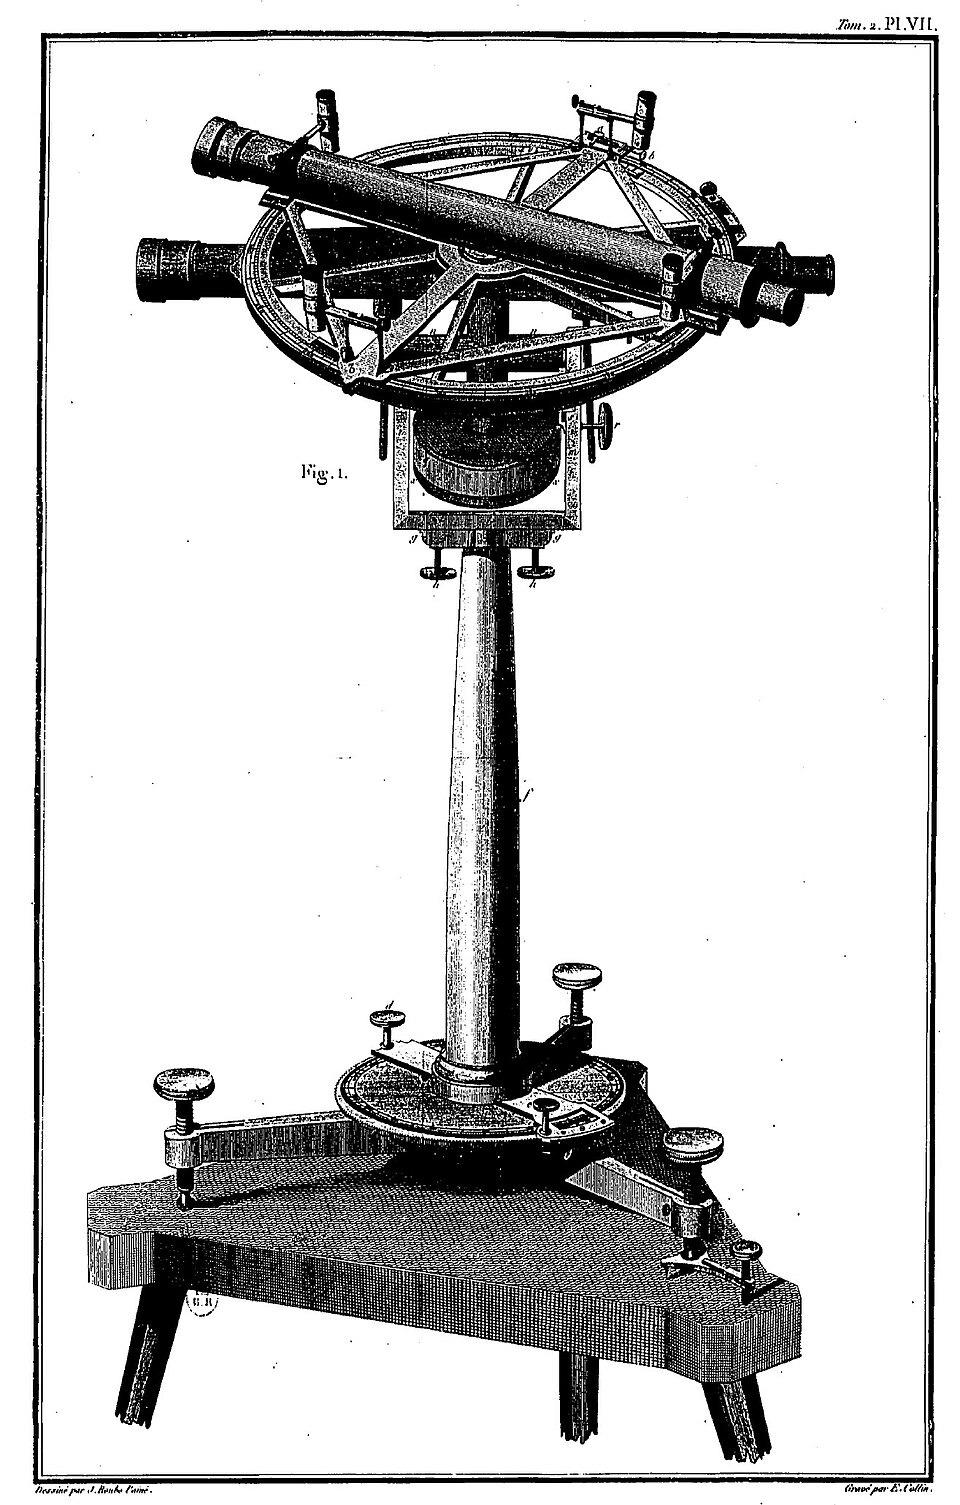
\includegraphics[width=0.3\linewidth]{images/book2/g10-delambre-repeating-circle.jpg}

{\small Lingkaran pengulang yang dipasang untuk mengukur sudut mendatar,
seperti diukir dalam laporan pengukuran Delambre (1807). Domain publik
(Wikimedia Commons).}
\end{center}
\end{history}

\section{Bumi yang pepat}

Sekitar tahun 1687, Isaac Newton berpendapat berdasarkan teori gravitasinya
bahwa Bumi yang berotasi pasti berbentuk sferoid yang pepat di kutub dan
menggembung di khatulistiwa. Pengukuran derajat meridian yang dilakukan para
astronom Observatorium Paris tampaknya menunjukkan sebaliknya: Bumi yang
memanjang ke arah kutub. Persoalan itu diselesaikan dengan mengukur panjang
satu derajat lintang di tempat-tempat yang sejauh mungkin satu sama lain.
% ledger: figure:expeditions

\begin{omfigure}
\begin{tikzpicture}[font=\small, >={Stealth[length=2mm]}]
  \def\a{3.0} \def\b{2.3}
  \draw[black!35, densely dashed] (0,0) circle (\a);
  \fill[omDef!8] (0,0) ellipse ({\a} and {\b});
  \draw[omDef!70!black, thick] (0,0) ellipse ({\a} and {\b});
  \draw[black!50] (-3.4,0) -- (3.7,0);
  \draw[black!50] (0,-2.6) -- (0,3.3);
  \draw[<->, omThm!85!black] (0,-0.3) -- (\a,-0.3);
  \node[omThm!85!black, below] at (1.5,-0.3) {$a$};
  \draw[<->, omThm!85!black] (-0.3,0) -- (-0.3,\b);
  \node[omThm!85!black, left] at (-0.3,1.15) {$b$};
  \node[above right] at (0,\b) {U};
  \node[anchor=south east] at (3.0,-2.5) {};
  \node[anchor=west] at (3.7,0) {khatulistiwa};
  % normal at t = 45 deg: P = (2.121, 1.626); crosses the equator at (0.874,0), the axis at (0,-1.14)
  \coordinate (P) at (2.121,1.626);
  \draw[omExo!85!black, thick] (P) -- ($(P)!1.35!(0.874,0)$);
  \draw[omExo!85!black, thick, ->] (P) -- ($(P)!-0.45!(0.874,0)$);
  \fill (P) circle (1.6pt);
  \node[anchor=west, align=left, font=\footnotesize] at (2.85,2.35) {vertikal setempat\\(unting-unting)};
  \draw[omExo!85!black] (1.45,0) arc (0:52.5:0.58);
  \node[omExo!85!black] at (1.62,0.32) {$\varphi$};
  \fill (0,0) circle (1.3pt);
  \node[anchor=north east, font=\footnotesize] at (0,0) {pusat};
  \node[black!50, font=\footnotesize, anchor=south] at (-2.2,2.15) {bola};
\end{tikzpicture}

{\small Bumi yang pepat, dengan \omterm{def:g10:measuring-the-earth:ellipsoid}{penggepengan} yang sangat dibesar-besarkan
(\omterm{def:g10:measuring-the-earth:ellipsoid}{penggepengan} yang sebenarnya terlalu kecil untuk terlihat pada skala ini).
Garis vertikal di suatu tempat tegak lurus pada permukaan; garis itu tidak
mengarah tepat ke pusat. Lintang $\varphi$ tempat itu adalah sudut antara
garis vertikalnya dan bidang khatulistiwa.}
\end{omfigure}

Lintang diukur dari bintang-bintang: lintang adalah sudut antara garis
vertikal setempat dan bidang khatulistiwa. Pada Bumi yang pepat, permukaan
dekat kutub kurang melengkung dibandingkan dengan dekat khatulistiwa. Di
tempat permukaan kurang melengkung, orang harus menempuh jarak yang lebih jauh
di sepanjang permukaan itu agar garis vertikal berputar satu derajat:
\emph{satu derajat lintang lebih panjang di dekat kutub}.

\begin{history}[Lapland dan Peru]
% ledger: figure:expeditions, figure:degrees
Pada 1735 Akademi Ilmu Pengetahuan Paris mengirim sebuah ekspedisi ke
khatulistiwa, di provinsi Spanyol Peru (kini Ekuador); ekspedisi itu bekerja
di sana selama sembilan tahun, sampai 1744. Pada 1736--1737 ekspedisi kedua, yang
dipimpin oleh Pierre-Louis Moreau de Maupertuis bersama matematikawan muda Alexis
Clairaut, mengukur satu derajat meridian di Lapland, dekat Lingkaran Arktik.
Derajat Lapland terukur 57\,437 \emph{toise} (satuan panjang lama; sekitar
\qty{111.95}{km}), sedangkan derajat Peru hanya 56\,737 toise: derajat lebih
panjang di dekat kutub, dan Newton benar. Kedua angka itu menunjukkan
\omterm{def:g10:measuring-the-earth:ellipsoid}{penggepengan} sekitar $1/205$ --- terlalu besar, seperti ditunjukkan
survei-survei selanjutnya, tetapi persoalan tandanya sudah terjawab.
\end{history}

\begin{omfigure}
\begin{tikzpicture}
\begin{axis}[omrecord, width=0.82\linewidth, height=5.4cm, xmin=0, xmax=90,
  ymin=110.45, ymax=111.8, xlabel={lintang (\unit{\degree})},
  ylabel={panjang \qty{1}{\degree} lintang (km)}, xtick={0,15,...,90},
  ytick={110.6,110.8,...,111.8}, yticklabel style={/pgf/number format/fixed, /pgf/number format/fixed zerofill, /pgf/number format/precision=1}]
\addplot[omDef!85!black, line width=1.1pt] table[x=lat_deg, y=deg_km] {figdata/out/grade-10-meridian_degree.dat};
\addplot[only marks, mark=*, mark size=1.8pt, omThm!85!black] coordinates {(0,110.574) (45,111.132) (66,111.507) (90,111.694)};
\node[anchor=south west, font=\footnotesize] at (axis cs:2,110.6) {110.57 km};
\node[anchor=north east, font=\footnotesize] at (axis cs:89,111.56) {111.69 km};
\node[anchor=north west, font=\footnotesize] at (axis cs:46,111.12) {111.13 km};
\node[anchor=south east, font=\footnotesize] at (axis cs:65,111.53) {111.51 km pada \ang{66} (Lapland)};
\end{axis}
\end{tikzpicture}

{\small Panjang satu derajat lintang pada \omterm{def:g10:measuring-the-earth:ellipsoid}{elipsoid referensi}
\cref{def:g10:measuring-the-earth:ellipsoid}, dari khatulistiwa sampai
kutub. Dihitung dari elipsoid WGS~84.}
\end{omfigure}

\begin{definition}[Elipsoid referensi dan penggepengan]\label{def:g10:measuring-the-earth:ellipsoid}
Yang disebut \emph{elipsoid referensi}\index{elipsoid referensi} adalah
permukaan yang diperoleh dengan memutar sebuah elips pada sumbu pendeknya,
yang dipilih agar sedekat mungkin dengan bentuk Bumi. Jari-jarinya di
khatulistiwa, yaitu \emph{jari-jari khatulistiwa}, adalah $a$, \emph{jari-jari
kutubnya} $b$, dan \emph{penggepengan}\index{penggepengan} elipsoid itu adalah
\[
  f = \frac{a-b}{a}.
\]
\end{definition}

\begin{proposition}[Ukuran-ukuran Bumi]\label{prop:g10:measuring-the-earth:dimensions}
% ledger: wgs84:ellipsoid, earth:Req, earth:Rpol, earth:Rmean (lengths computed in figdata/grade-10/meridian_degree.py)
\omterm{def:g10:measuring-the-earth:ellipsoid}{Elipsoid referensi} yang dipakai penentuan posisi dengan satelit (WGS~84) memiliki
\[
  a = \qty{6378.137}{km}, \qquad b = \qty{6356.752}{km}, \qquad
  f = \frac{1}{298.257}.
\]
Jari-jari kutub \qty{21.4}{km} lebih pendek daripada jari-jari khatulistiwa.
Panjang khatulistiwa \qty{40075}{km}, sedangkan meridian, dari kutub ke kutub
dan kembali lagi, \qty{40008}{km}; seperempat meridian, dari khatulistiwa ke
sebuah kutub, panjangnya \qty{10001.966}{km}. Satu derajat lintang panjangnya
\qty{110.574}{km} di khatulistiwa dan \qty{111.694}{km} di kutub. Satu
derajat bujur panjangnya \qty{111.32}{km} di khatulistiwa dan memendek ke arah
kutub kira-kira sebanding dengan $\cos \varphi$.
\end{proposition}

\begin{example}[Satu derajat bujur]\label{ex:g10:measuring-the-earth:longitude}
Paralel pada lintang $\varphi$ adalah lingkaran yang jari-jarinya sama dengan
jaraknya dari sumbu, sekitar $R \cos \varphi$. Pada \qty{60}{\degree} LU
kelilingnya sekitar setengah keliling khatulistiwa, dan satu derajat bujur
panjangnya sekitar $111.32 \times \cos 60^\circ \approx \qty{55.7}{km}$
(elipsoid memberikan \qty{55.80}{km}).
\end{example}

\begin{remark}[Seberapa bulatkah bulat itu?]\label{rem:g10:measuring-the-earth:round}
\omterm{def:g10:measuring-the-earth:ellipsoid}{Penggepengan} sebesar $1/298$ itu kecil. Pada bola dunia bergaris tengah
\qty{30}{cm}, diameter kutubnya hanya \qty{1}{mm} lebih pendek daripada
diameter khatulistiwanya --- tak terlihat. Palung samudra terdalam, hampir
\qty{11}{km} di bawah permukaan laut, hanya akan menjadi goresan sedalam
kira-kira seperempat milimeter. Untuk sebagian besar keperluan, Bumi adalah
bola dengan jari-jari rata-rata \qty{6371}{km}; untuk posisi yang teliti,
elipsoid diperlukan.
% ledger: earth:Rmean, usgs:trench-depth
\end{remark}

\section{Geodesi masa kini}

\begin{omfigure}
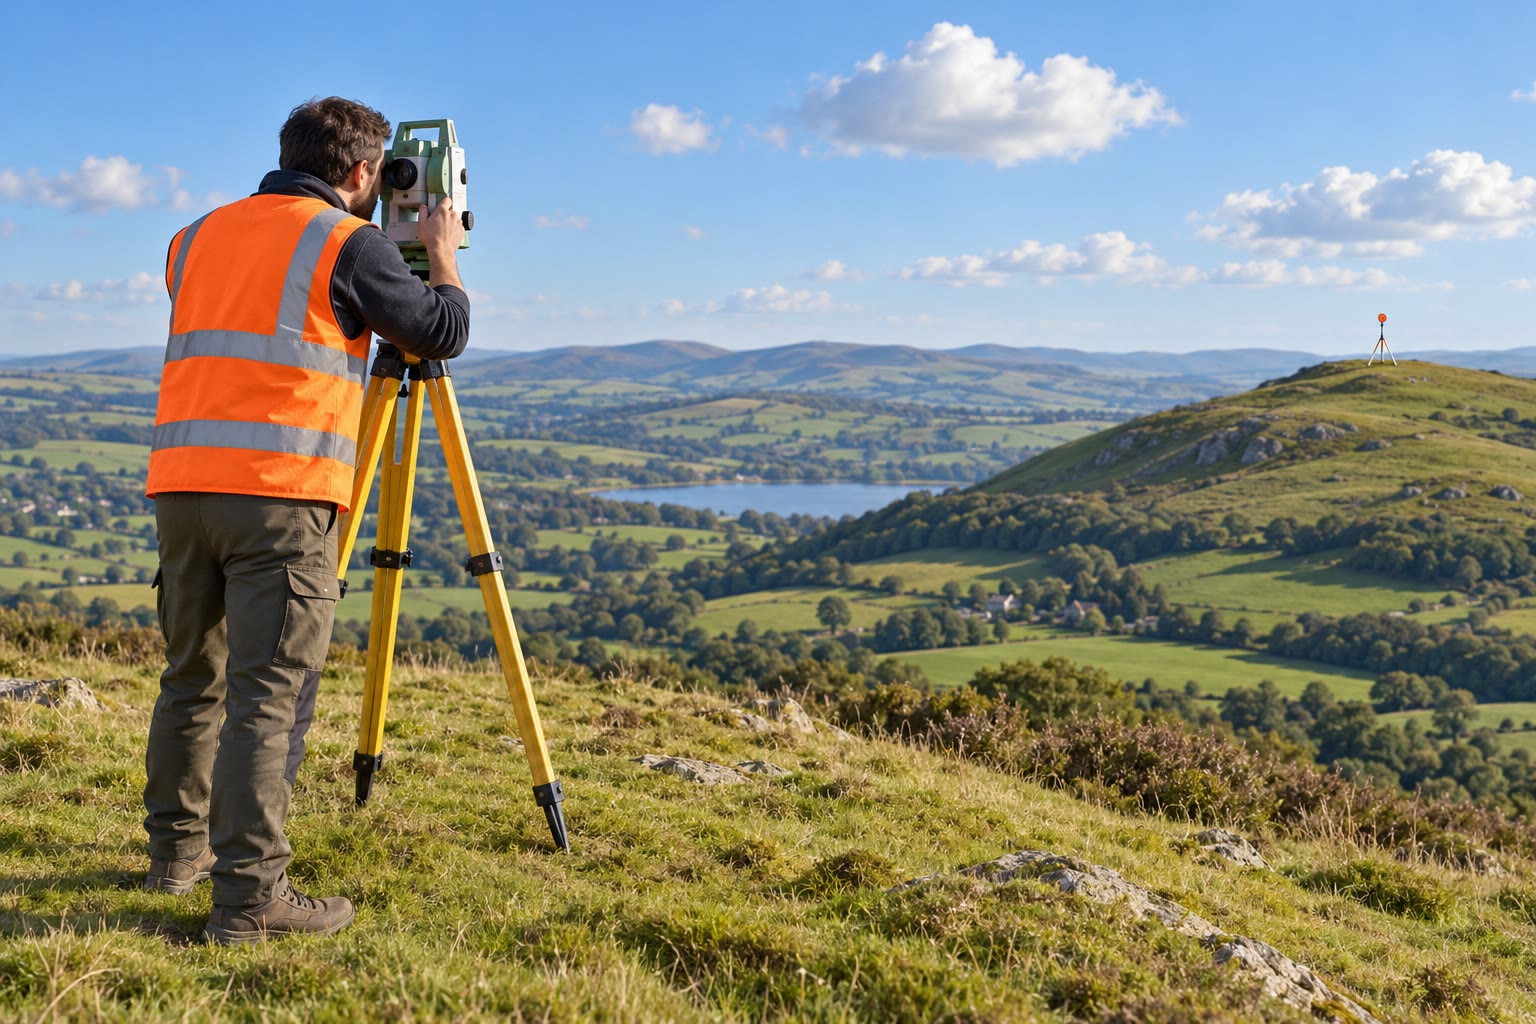
\includegraphics[width=0.7\linewidth]{images/book2/ai/g10-surveyor-theodolite.jpg}

{\small Seorang juru ukur bekerja dengan alat modern yang mengukur sudut dan,
dengan seberkas cahaya, juga jarak; sebuah tanda survei berdiri di bukit di
seberang.}
\end{omfigure}

\omterm{def:g10:measuring-the-earth:triangulation}{Triangulasi-triangulasi} besar abad kedelapan belas dan kesembilan belas kini
telah digantikan oleh satelit. Sebuah penerima di tanah menangkap sinyal dari
beberapa satelit yang posisinya diketahui setiap saat, lalu menghitung
posisinya sendiri dari waktu tempuh sinyal-sinyal itu (Buku 1). Jaringan
penerima tetap, yang dipasang pada batuan dasar di seluruh dunia, mengukur
posisinya terus-menerus. Jaringan itu menetapkan kerangka acuan tempat setiap
peta dan setiap posisi satelit dinyatakan, dan jaringan itu bergerak:
penerima-penerimanya memperlihatkan lempeng-lempeng litosfer yang bergeser
beberapa sentimeter per tahun (\cref{ch:g11:plate-motions}).
% ledger: usgs:gps

\begin{inthefield}[Mengukur tanah masa kini]
Para ahli \omterm{def:g10:measuring-the-earth:geodesy}{geodesi} memasang antena pada tiang beton yang ditanam di batuan
dasar, jauh dari bangunan dan pepohonan, dan merekam posisinya setiap beberapa
detik selama bertahun-tahun. Mereka menggabungkan rekaman itu dengan
pengukuran teleskop radio yang mengamati galaksi-galaksi yang sangat jauh dan
dengan sinar laser yang ditembakkan ke satelit-satelit bercermin. Para juru
ukur di lokasi pembangunan dan di pedesaan masih mengukur sudut dan jarak
dengan alat bertripod, lalu mengikatkannya pada kerangka satelit.
\end{inthefield}

\section{Latihan}

\begin{exercise}[$\star$]\label{exo:g10:measuring-the-earth:1}
Sebutkan tiga pengamatan, yang dapat dilakukan tanpa meninggalkan permukaan
tanah, yang menunjukkan bahwa Bumi itu bulat. Untuk masing-masing, jelaskan
dalam satu kalimat mengapa Bumi yang datar tidak dapat menghasilkannya.
\end{exercise}

\begin{exercise}[$\star$]\label{exo:g10:measuring-the-earth:2}
Apa itu \omterm{def:g10:measuring-the-earth:geodesy}{geodesi}? Apa itu \omterm{def:g10:measuring-the-earth:triangulation}{triangulasi}, dan satu-satunya panjang apa yang harus
diukur di tanah dalam sebuah \omterm{def:g10:measuring-the-earth:triangulation}{triangulasi}?
\end{exercise}

\begin{exercise}[$\star$]\label{exo:g10:measuring-the-earth:3}
Eratosthenes mendapati bahwa sudut antara sinar Matahari dan garis vertikal
di Aleksandria adalah $1/50$ lingkaran penuh ketika Matahari tepat di atas
kepala di Syene, yang berjarak 5000 stadion. Hitung kelilingnya dalam stadion,
lalu dalam kilometer, dengan satu stadion \qty{157.2}{m}.
\end{exercise}

\begin{exercise}[$\star$]\label{exo:g10:measuring-the-earth:4}
Satu derajat lintang panjangnya sekitar \qty{111}{km}. Berapa panjang satu
menit lintang ($1/60$ derajat)? Kira-kira berapa panjang meridian dari
khatulistiwa sampai kutub?
\end{exercise}

\begin{exercise}[$\star$]\label{exo:g10:measuring-the-earth:5}
Dengan jari-jari khatulistiwa \qty{6378.137}{km} dan jari-jari kutub
\qty{6356.752}{km}, hitung selisih kedua jari-jari itu dan \omterm{def:g10:measuring-the-earth:ellipsoid}{penggepengan}
$f = (a-b)/a$. Nyatakan $f$ sebagai satu dibagi sebuah bilangan bulat.
\end{exercise}

\begin{exercise}[$\star\star$]\label{exo:g10:measuring-the-earth:6}
Dua kota terletak pada meridian yang sama, berjarak \qty{500}{km}. Pada tengah
hari di hari yang sama, sebatang tongkat tegak setinggi \qty{1.00}{m}
membentuk bayang-bayang \qty{0.364}{m} di kota yang di selatan dan
\qty{0.456}{m} di kota yang di utara. Hitung sudut antara sinar Matahari dan
garis vertikal di setiap kota, lalu keliling Bumi.
\end{exercise}

\begin{exercise}[$\star\star$]\label{exo:g10:measuring-the-earth:7}
Dalam segitiga $ABC$, garis dasar $AB = \qty{10.00}{km}$, sudut di $A$
\qty{62}{\degree}, dan sudut di $B$ \qty{71}{\degree}. Hitung sudut di $C$
serta panjang $AC$ dan $BC$.
\end{exercise}

\begin{exercise}[$\star\star$]\label{exo:g10:measuring-the-earth:8}
Sebuah pesawat terbang tepat ke arah barat sepanjang paralel
\qty{60}{\degree} LU, dari bujur \qty{10}{\degree} BT ke bujur
\qty{20}{\degree} BB. Dengan panjang satu derajat bujur $111.3 \cos \varphi$
km, hitung jarak yang ditempuhnya. Berapa panjang perubahan bujur yang sama
di khatulistiwa?
\end{exercise}

\begin{exercise}[$\star\star$]\label{exo:g10:measuring-the-earth:9}
Mata seorang pengamat berada $h = \qty{2}{m}$ di atas laut yang tenang. Garis
pandang ke cakrawala menyinggung laut di $T$; pusat Bumi adalah $O$, dan mata
pengamat $E$. Jelaskan mengapa segitiga $OTE$ siku-siku di $T$, lalu gunakan
teorema Pythagoras dengan $R = \qty{6371}{km}$ untuk menunjukkan bahwa jarak
ke cakrawala kira-kira $\sqrt{2Rh}$, dan hitung jarak itu.
\end{exercise}

\begin{exercise}[$\star\star$]\label{exo:g10:measuring-the-earth:10}
Bacalah kurva panjang derajat. Di antara lintang berapa panjang satu derajat
berubah paling cepat? Jelaskan dalam dua kalimat mengapa satu derajat lintang
lebih panjang di dekat kutub daripada di dekat khatulistiwa.
\end{exercise}

\begin{exercise}[$\star\star$]\label{exo:g10:measuring-the-earth:11}
Busur meridian dari Dunkirk ke Barcelona meliputi \qty{9.646}{\degree}
lintang dan panjangnya \qty{1072.2}{km}. Hitung panjang rata-rata satu derajat
di sepanjang busur itu. Jika setiap derajat sepanjang itu, berapa panjang
seperempat meridian? Bandingkan dengan \qty{10002.0}{km} dan jelaskan selisih
kecil itu.
\end{exercise}

\begin{exercise}[$\star\star\star$]\label{exo:g10:measuring-the-earth:12}
Eratosthenes mengukur sudut \qty{7.2}{\degree} dan jarak 5000 stadion. Jika
sudutnya keliru sebesar \qty{0.1}{\degree} (terlalu kecil), berapa persen
kesalahan kelilingnya, dan ke arah mana? Menurutmu, manakah di antara kedua
pengukurannya yang kurang teliti?
\end{exercise}

\begin{exercise}[$\star\star\star$]\label{exo:g10:measuring-the-earth:13}
Rantai dua segitiga: pada $ABC$, $AB = \qty{6.000}{km}$,
$A = \qty{55}{\degree}$, $B = \qty{75}{\degree}$. Pada segitiga berikutnya
$ACD$, yang dibangun pada sisi $AC$, sudut di $A$ \qty{50}{\degree} dan sudut
di $C$ \qty{68}{\degree}. Hitung $AC$, lalu $AD$.
\end{exercise}

\begin{exercise}[$\star\star\star$]\label{exo:g10:measuring-the-earth:14}
Pada lintang berapa panjang satu derajat bujur setengah panjangnya di
khatulistiwa? Pada lintang berapa sepersepuluhnya? Jelaskan mengapa kedua
jawaban itu tidak bergantung pada ukuran Bumi.
\end{exercise}

\begin{exercise}[$\star\star\star$]\label{exo:g10:measuring-the-earth:15}
Gunakan nilai-nilai elipsoid: satu derajat lintang panjangnya
\qty{110.574}{km} di khatulistiwa dan \qty{111.694}{km} di kutub. Pada bola
dengan jari-jari rata-rata yang sama, satu derajat akan sepanjang
\qty{111.195}{km} di mana-mana. Berapa meter kesalahan seorang juru ukur yang
menganggap Bumi bola, untuk satu derajat di khatulistiwa, dan untuk satu
derajat di kutub? Mengapa peta yang memberikan posisi sampai ketelitian meter
harus dihitung pada elipsoid?
\end{exercise}

\section{Soal: Meter dan Meridian}

\begin{problem}[{Soal akhir pekan --- dari bayang-bayang Eratosthenes sampai
panjang meter yang pertama}]
\label{pb:g10:measuring-the-earth:1}
% ledger: geonames:aswan, geonames:alexandria, erat:method, metre:1791, metre:survey, wgs84:ellipsoid (arc lengths and degree lengths computed in figdata/grade-10/meridian_degree.py)
Seorang siswa menelusuri kembali sejarah pengukuran Bumi dengan angka-angka
modern. Aswan, Syene zaman kuno, terletak pada lintang
\qty{24.09}{\degree} LU dan Aleksandria pada \qty{31.20}{\degree} LU; pada
elipsoid modern, busur meridian di antara kedua paralelnya panjangnya
\qty{788}{km}. Pada elipsoid, satu derajat lintang panjangnya
\qty{110.57}{km} di khatulistiwa, \qty{111.13}{km} pada \qty{45}{\degree},
dan \qty{111.51}{km} pada \qty{66}{\degree}, sedangkan seperempat meridian
panjangnya \qty{10001.966}{km}.

\medskip
\noindent\textbf{Bagian I --- Eratosthenes sekali lagi.}
\begin{enumerate}
  \item Hitung selisih lintang antara Aswan dan Aleksandria.
  \item Berapa bagian lingkaran penuh selisih itu? Bandingkan dengan $1/50$
        milik Eratosthenes.
  \item Hitung keliling Bumi yang diberikan metode Eratosthenes dengan
        angka-angka modern ini.
  \item Kedua kota itu tidak terletak pada meridian yang sama: Aswan berada
        sekitar \qty{3}{\degree} bujur di sebelah timur Aleksandria. Jarak
        mana yang harus dipakai dalam metode ini: jarak lurus antara kedua
        kota atau busur meridian di antara paralel-paralelnya? Mengapa?
  \item Mengapa kedua bayang-bayang harus diukur pada hari yang sama, pada
        tengah hari setempat?
\end{enumerate}

\medskip
\noindent\textbf{Bagian II --- Triangulasi kecil.}
Sebuah garis dasar $AB = \qty{12.000}{km}$ diukur. Dari $A$, tanda $C$
terlihat \qty{58}{\degree} dari $B$; dari $B$, \qty{66}{\degree} dari $A$.
Pada segitiga berikutnya $ACD$, sudut di $A$ \qty{47}{\degree} dan sudut di
$C$ \qty{75}{\degree}. Sisi $AD$ mengarah \qty{8}{\degree} ke timur dari arah
utara.
\begin{enumerate}[resume]
  \item Hitung sudut di $C$ pada segitiga $ABC$.
  \item Hitung sisi $AC$.
  \item Hitung sisi $BC$.
  \item Hitung sudut di $D$ pada segitiga $ACD$, lalu sisi $AD$.
  \item Hitung jarak utara--selatan antara $A$ dan $D$.
  \item Dengan panjang derajat pada \qty{45}{\degree}, hitung selisih
        lintang antara $A$ dan $D$, dalam derajat dan dalam menit busur.
\end{enumerate}

\medskip
\noindent\textbf{Bagian III --- Bumi yang pepat.}
\begin{enumerate}[resume]
  \item Berapa meter satu derajat lintang pada \qty{66}{\degree} lebih
        panjang daripada satu derajat di khatulistiwa?
  \item Jelaskan apa yang ditunjukkan selisih ini tentang bentuk Bumi.
  \item Pada elipsoid, $a = \qty{6378.137}{km}$ dan
        $b = \qty{6356.752}{km}$. Hitung $a - b$ dan \omterm{def:g10:measuring-the-earth:ellipsoid}{penggepengannya}.
  \item Jelaskan mengapa, pada Bumi yang pepat, garis unting-unting di tempat
        berlintang \qty{45}{\degree} tidak mengarah tepat ke pusat
        Bumi.
\end{enumerate}

\medskip
\noindent\textbf{Bagian IV --- Meter yang pertama.}
\begin{enumerate}[resume]
  \item Menurut definisi tahun 1791, berapa seharusnya panjang seperempat
        meridian, dalam meter?
  \item Meter platina tahun 1799 dibuat dari nilai meridian yang terukur.
        Jika seperempat meridian sebenarnya \qty{10001.966}{km}, berapa
        panjang sepersepuluh jutanya?
  \item Apakah meter tahun 1799 terlalu panjang atau terlalu pendek
        dibandingkan dengan definisinya sendiri? Sebesar berapa bagian?
  \item Batang platina itu menyalin dengan setia panjang yang dihitung pada
        tahun 1790-an. Apakah seperempat meridian yang dihitung saat itu
        terlalu panjang atau terlalu pendek? Jelaskan.
  \item Berapa milimeter meter yang pertama lebih pendek daripada
        sepersepuluh juta seperempat meridian yang sebenarnya? Bandingkan
        dengan tebal selembar kertas, sekitar \qty{0.1}{mm}.
\end{enumerate}
\end{problem}
